\documentclass{article}
\usepackage{amsfonts}
\usepackage{amsmath}
\usepackage{xcolor}

\usepackage{enumitem}

\usepackage{graphicx}
\graphicspath{{./images/}}
\usepackage{sidecap}

\usepackage{hyperref}

\usepackage{listings}
% \lstset{
%   % basicstyle=\ttfamily,
%   % columns=fullflexible,
%   % frame=single,
%   breaklines=true,
%   postbreak=\mbox{\textcolor{red}{$\hookrightarrow$}\space}
% }
\lstset{
  basicstyle=\ttfamily,
  breaklines=true,
  postbreak=\mbox{\textcolor{red}{$\hookrightarrow$}\space},
  numbers=left,
  stepnumber=1,
  tabsize=1,
}

\usepackage[margin=1in]{geometry}

\usepackage{float}

\title{Real-Time Procedural Terrain Generation with Marching Cubes}
\author{Joseph Chambers-Graham}
\date{}

\setcounter{tocdepth}{3}

\begin{document}

\bibliographystyle{plainurl}

\maketitle
\newpage

\section*{Abstract}
This project explores a method for procedurally generating terrain by applying the a variation of the Marching Cubes algorithm known as the Transvoxel algorithm. We use an octree data structure to break down a large world into chunks at varying levels of detail, and apply the parallel processing power of the GPU to rapidly generate geometry on a per-chunk basis. We then explore applications of this approach, modifying the geometry in real-time by making localized changes to the underlying distance function. %Finally, we demonstrate the applicability of this approach by 
Finally, we use the meshes we have generated with a well-known physics library.
\newpage

\tableofcontents

\newpage
\section{Introduction}
- project and report overview
\section{Background}
\subsection{Signed Distance Functions}
\label{section:sdf}
At the core of the Marching Cubes algorithm, and the way we will be defining shapes, is the signed distance function (SDF). This is a function of the form $f:\mathbb{R}^3 \rightarrow \mathbb{R}$. The shape represented by an SDF is the implicit surface $f\left(x,y,z\right) = 0$. Furthermore, it is desirable for an SDF to have the following properties:
\begin{enumerate}[label=\roman*.]
\item At all points where $f\left(x,y,z\right) \neq 0$, if $\left(x,y,z\right)$ is inside the surface, $f\left(x,y,z\right) < 0$. If $\left(x,y,z\right)$ is outside the surface, $f\left(x,y,z\right) > 0$. This is the most important property of an SDF, without which the Marching Cubes algorithm is unlikely to produce valid geometry.
\item At all points where $f\left(x,y,z\right) \neq 0$, the value $f\left(x,y,z\right)$ should be the smallest (signed) euclidean distance from the point $\left(x,y,z\right)$ to the surface $f\left(x,y,z\right) = 0$. In practice, many implicit functions we are using do not have this property, however for best results the value $f\left(x,y,z\right)$ should be a good approximation of the actual distance, and for floating point precision reasons, must be at least the same order of magnitude. This property will be used by the Marching Cubes algorithm to interpolate the positions of vertices, and as such a better distance approximation will lead to a more accurate mesh representation of the SDF. An SDF such that $f\left(x,y,z\right)$ gives the correct distance everywhere is an \textit{exact} SDF. Otherwise, it is an \textit{approximate} SDF.
\item $f$ is continuous everywhere, and has all partial derivatives. This is useful for calculating the normal to the surface at a given point. In practice, we will relax these restrictions, but this should still hold in places where the algorithm might generate vertices.
\end{enumerate}
Many primitive shapes have exact SDF representations \cite{quilez:sdf}. Figure \ref{fig:Circle_SDF} shows a 2 dimensional exact SDF for a circle.

\begin{SCfigure}[][h]
\caption{Example of a 2 dimensional SDF representing a circle. The function shown is $f\left(x,y\right) = \sqrt{x^2+y^2}-1$, with the area where $f\left(x,y\right) < 0 $ shaded. Also shown are the contours where $f\left(x,y\right) = 0.1,0.2,...0.5$}
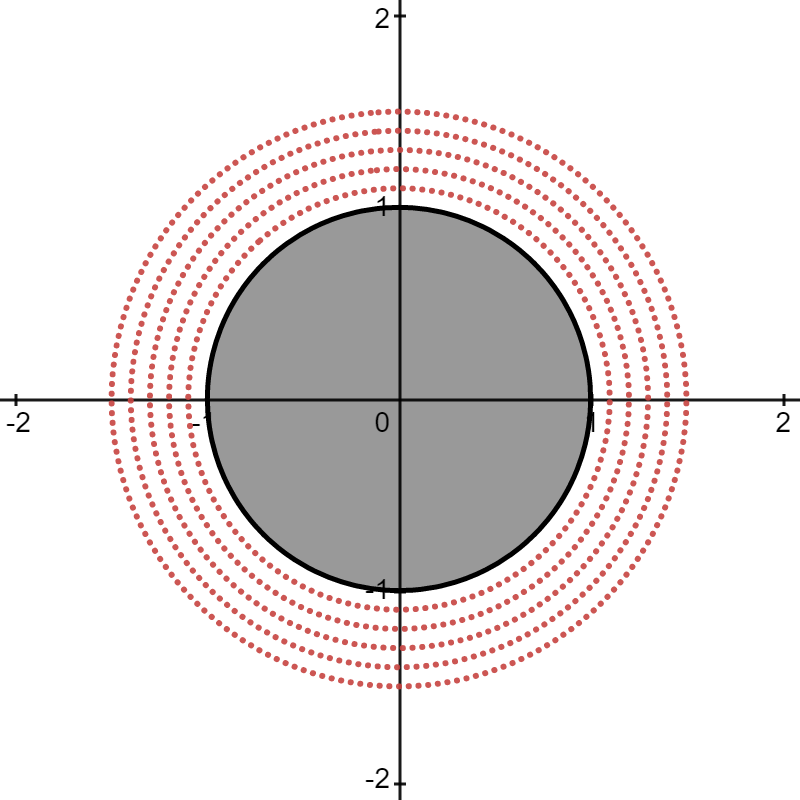
\includegraphics[width=0.5\textwidth]{Circle_SDF}
\label{fig:Circle_SDF}
\end{SCfigure}

However, many useful shapes, in particular heightmaps and shapes those defined by random noise, are not easy to represent as an exact SDF. For this sort of shape, we use an approximate SDF. Figure \ref{fig:Hill_SDF} shows a 2 dimensional approximate SDF for the heightmap defined by $y=1-\frac{x^2}{3}$. It is of course possible to define the exact distance function for any implicit shape, however such problems are often minimisation problems with with solutions that are expensive to compute. For example,even this simple example computing the exact distance to a quadratic curve requires computing the roots of a cubic polynomial, and computing the exact distance to a cubic curve requires solving a polynomial of degree 5, for which there is no elementary solution. Since this is useful for defining shapes based on interpolation splines, it is certainly worth considering when an approximation may be worth using due to the reduced computational cost.

\begin{SCfigure}[][h]
\caption{Plot of the SDF $f\left(x,y\right) = y - \left(1 - \frac{x^2}{3}\right)$. Note the contour lines are no longer uniformly spaced, as they would be with an exact SDF. In fact, the distance approximation gets worse, as the slope of the surface increases.}
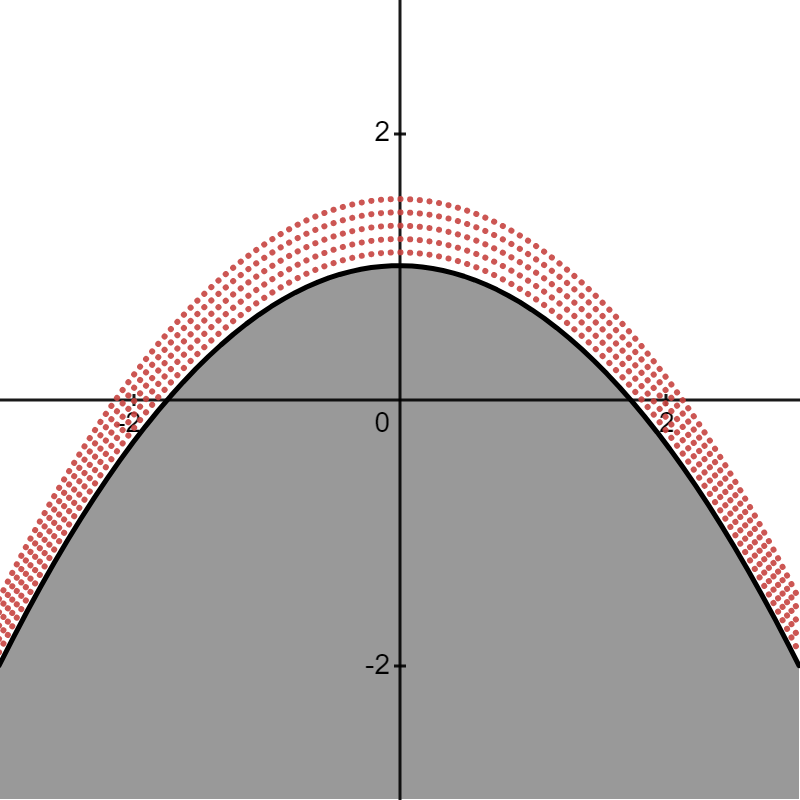
\includegraphics[width=0.5\textwidth]{Hill_SDF}
\label{fig:Hill_SDF}
\end{SCfigure}

The basic set-theoretical operations of union, intersection, and difference have equivalent representations using the $\min$ and $\max$ functions. At this point, one many note that the function $\min\left(f,g\right)$ may fail to be differentiable at the point where $f = g$. Here, we may simply take the derivative of $f$ or $g$. 
\\
It is worth noting that some literature chooses the terminology of signed \textit{density} functions \cite{nguyen_geiss_2007}. This is equivalent to an approximate SDF, however the sign convention is flipped, so that a negative value is outside the surface.\\
%https://developer.nvidia.com/gpugems/gpugems3/part-i-geometry/chapter-1-generating-complex-procedural-terrains-using-gpu

\subsection{Noise}
A typical noise function takes as input a point in $\mathbb{R}^n$ and returns a pseudorandom value, usually between 0 and 1. The use of noise to generate convincing heightmaps is well-documented, and typical implementations are as a function of the form $y = h\left(x,z\right)$ giving the height of the terrain at a given $\left(x,z\right)$ coordinate. This can be simply extended to an approximate SDF, using the formula $f\left(x,y,z\right) = y - h\left(x,z\right)$. Note that this is in fact an approximate SDF, and that the distance approximation worsens as the steepness of the slope of $h\left(x,z\right)$ increases. This phenomenon can be seen in figure \ref{fig:Hill_SDF}.
\\
The use of 3 dimensional noise as a distance function is also possible, and yields interesting results. %TODO - implement  this

\subsection{Marching Cubes Algorithm}
\label{section:mc}
The Marching Cubes algorithm is an algorithm for polygonising a 3 dimensional scalar field. It works by splitting the space into a uniform grid of cubes (\textit{cells}), and sampling the scalar field at the vertices of each cube. Pre-computed lookup tables, indexed by the vertices of the cell which are classified as "inside" or "outside", are used to determine the geometry that exists within the cell. Each vertex of this geometry lies on an edge of the cell, and the position of each geometry vertex is adjusted by linearly interpolating the sampled values of the scalar field at the cell vertices, such that the vertex is placed approximately on the surface described by the scalar field. In this project, we use a 3 dimensional SDF as described in Section \ref{section:sdf} to provide scalar field samples, and the lookup tables as described by Paul Bourke. \cite{bourke_1994}

\section{Design}
\subsection{GPU Implementation}
\label{section:mc_gpu}
The Marching Cubes algorithm operates on a large grid of cells, on a per-cell basis. As such, it is well-suited to parallelisation. In this section, we describe an implementation of the Marching Cubes algorithm on a GPU, using GLSL. This implementation is based on the reference implementation cited in Section \ref{section:mc}. The implementation works on \textit{chunks}, which are cuboids of grid cells, and is split into 3 phases:
\begin{enumerate}

\item \underline{Distance function computation}: For each grid cell vertex in the chunk, the SDF is sampled, and the values are stored in a buffer to be passed to the subsequent phases. This is done separately to the other phases, which operate over grid cells rather than grid cell vertices, to avoid unnecessary recomputation of the SDF, since one grid cell vertex may belong to up to 8 neighboring grid cells.
\begin{lstlisting}[language=C++,label={mc_generate},caption={GLSL code for generating the SDF at one vertex in a chunk. The function \texttt{generate} may use any SDF, and stores the value in a buffer.}]
void main() {
  uvec3 gid = gl_GlobalInvocationID;
  if (gid.x > chunkSize.x || gid.y > chunkSize.y || gid.z > chunkSize.z) {
    return;
  }
  generate(gid);
}
\end{lstlisting}

\item \underline{Counting phase}: For each grid cell in the chunk, the number of mesh triangles in the cell is calculated, using the SDF sample values computed in the previous phase. This allows the vertex buffer to be sized correctly. This phase also filters out grid cells which have no triangles in at all, since no geometry needs to be generated. Listing \ref{mc_count} shows part of the code responsible for this. Variable \texttt{cubeIndex} is calculated according to the Marching Cubes algorithm, and corresponds to the vertices of the grid cell that are inside or outside of the surface. Hence, this \textit{cube index} determines the geometry that will end up in each grid cell. \texttt{totalTable} contains the number of triangles in a grid cell with that index, which is added to the atomic variable \texttt{pointCount}. \texttt{bufferIndex} reserves a place in the buffer \texttt{marchableList} for this grid cell. The condition in line 1 filters out the cube indices which do not generate any geometry.
\begin{lstlisting}[language=C++,label={mc_count},caption={GLSL code for counting the number of vertices and marchable grid cells in the chunk.}]
if (cubeIndex != 0 && cubeIndex != 255)
{
  atomicCounterAddARB(pointCount,totalTable[cubeIndex]);
  uint bufferIndex = atomicCounterIncrement(marchableCount);
  uvec4 mc = uvec4(gid.x,gid.y,gid.z,cubeIndex);
  marchableList[bufferIndex] = mc;
}
\end{lstlisting}

\item \underline{Polygonisation phase}: For each of the grid cells that will contain mesh triangles, these triangles are actually generated, and the vertex positions are adjusted by linearly interpolating the pre-computed SDF values. At this stage, the vertex normals are also generated. This can be done using face normals, or by providing a normal function. Listing \ref{mc_poly} shows part of the code responsible for this. Atomic variable \texttt{triCount} keeps track of the number of triangles that have been generated across the entire chunk, and allocates a space in the buffers \texttt{vertices} and \texttt{normals}, which have been sized according to the values calculated in the previous phase. \texttt{triTable} is a buffer containing a flattened version of the table with the same name in the reference implementation. It contains a list of indices into the array \texttt{vertlist} for each cube index. Each vertex in \texttt{vertlist} is positioned on the edge of the grid cell, linearly interpolated as described in Section \ref{section:mc}.
\begin{lstlisting}[language=C++,label={mc_poly},caption={GLSL code for generating the geometry of a grid cell.}]
for (int tCount = 0; triTable[tCount+16*cubeIndex] != -1; tCount+=3)
{
  uint index = atomicCounterIncrement(triCount);
  for (int t = 0; t < 3;t++)
  {
    vec3 vertPos = vertlist[triTable[cubeIndex*16+tCount+t]]*chunkStride + chunkPosition;
    vertices[3*index+t] = vec4(vertPos,1);
    normals[3*index+t] = vec4(modified_normal(vertPos),0);
  }
}
\end{lstlisting}

\end{enumerate}
The choice to parallelise the algorithm in this way presents some downsides. Triangles are generated and placed into the vertex buffer in an order which is very unlikely to be coherent, meaning that there is no way to reliably use an index buffer for vertices that are generated in the same place, a common occurance. This results in many duplicate vertices in the vertex array. Nevertheless, this is a worthwhile tradeoff, with the GPU implementation greatly outperforming the CPU implementation. 
\subsubsection{Comparison of CPU and GPU implementations}
The SDF used for these comparison tests is a scaled 3D noise function. Pseudorandom numbers for this noise function are generated using combinations of built in floating point functions in GLSL in the GPU implementation, and functions from the GLM C++ library in the CPU implementation. An effort has been made to ensure these functions are equivalent, however due to floating point inaccuracies and differences between these implementations, the SDF occasionally produces slightly different values between implementations, and this results in the number of triangles generated being slightly different also. However, this difference is very small compared to the total number of triangles generated, so is unlikely to have a significant impact on the runtime comparison. For example, the largest test, generating 1000 chunks of size $32^3$, produces 4394195 triangles on the CPU, and 4394045 on the GPU.
Table \ref{tab:cpu-gpu-comparison} shows the time taken to generate different numbers of chunks of 3D noise, of size $32^3$, using the reference CPU implementation, and this GPU implementation. All experiments were run using an Intel i9-9900k and Nvidia RTX 2080ti. Each experiment was run 5 times, and the average time is shown.
\begin{table}[H]
  \begin{tabular}{|c|c|c|c|}
    \hline
    Test & Approximate Triangle Count & CPU Time (ms) & GPU Time (ms) \\
    \hline
    \hline
    1 Chunk & 1k & 65.4 & 4.2\\
    4x4x4 Chunks & 240k & 6817.4 & 60.8\\
    10x1x10 Chunks & 500k & 12650.2 & 90.0\\
    10x10x10 Chunks & 4.4M & 117568.6 & 635.0\\
    \hline
    
  \end{tabular}
  \caption{\label{tab:cpu-gpu-comparison}Performance comparison between the CPU and GPU implementations}
\end{table}

\begin{figure}[H]
  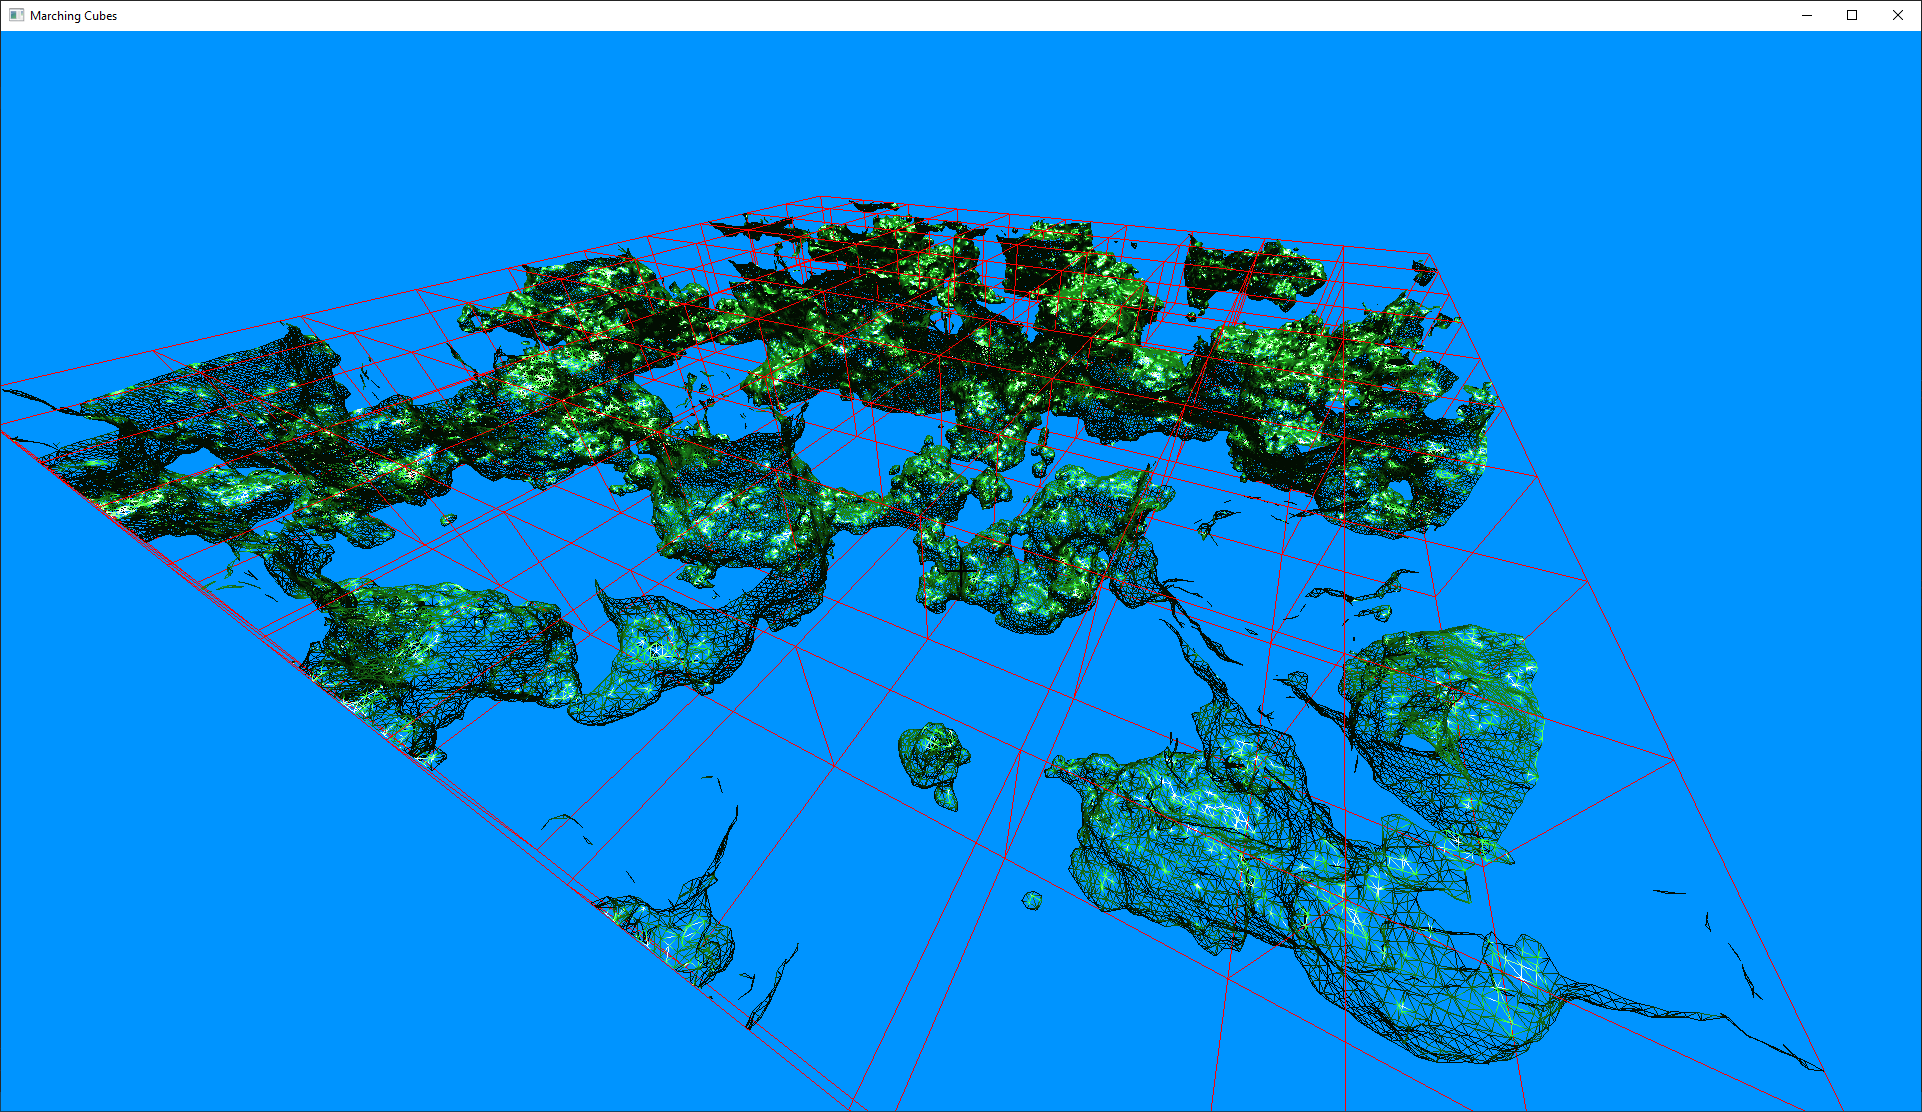
\includegraphics[width=\textwidth]{10x10_wireframe.png}
  \caption{An example of the 3D noise generated by these tests. This figure shows a wireframe of the 10x1x10 chunk test, with backface culling enabled.}
\end{figure}

\subsection{LOD system}
Even with a much more efficient GPU implementation of the Marching Cubes algorithm, when attempting to generate very large areas of geometry, it becomes infeasible to generate and render a uniform grid of Marching Cubes chunks. Furthermore, generating large amounts of triangles very far away from the camera is unnecessary, since the detail will not be visible. For this reason, it is necessary to have a dynamic level of detail (LOD) system.

\subsubsection{Octree}
\label{section:octree}
To implement a versatile LOD system, an octree data structure is used. %TODO - explain an octree?
Each octree node represents a cuboid of space, such that the root node of the octree represents the entire renderable world, and the 8 children of an octree node equally divide the space represented by the parent node into octants. Each leaf node contains a reference to a chunk of generated geometry, as described in section \ref{section:mc_gpu}. The depth of the octree in any given region corresponds to the level of detail at which that region will have geometry generated. Each Marching Cubes chunk is generated with the same number of grid cells, regardless of the level of detail it is being generated for. However, the size of the grid cells doubles for each detail level increase. Using an octree provides versatility since any condition can be used to set the level of detail at a specific point in space. For example, it will be desirable to use the maximum level of detail near physics objects, so the physics collision is as accurate as possible, even if the camera is very far away. These conditions will be represented by functions \texttt{shouldSplit} and \texttt{shouldChop} for each node in the octree. The function \texttt{shouldSplit} returns whether a leaf node should split into its 8 children, and \texttt{shouldChop} returns whether a non-leaf node, should become a leaf, removing the rest of the octree below that node.

\begin{figure}[H]
  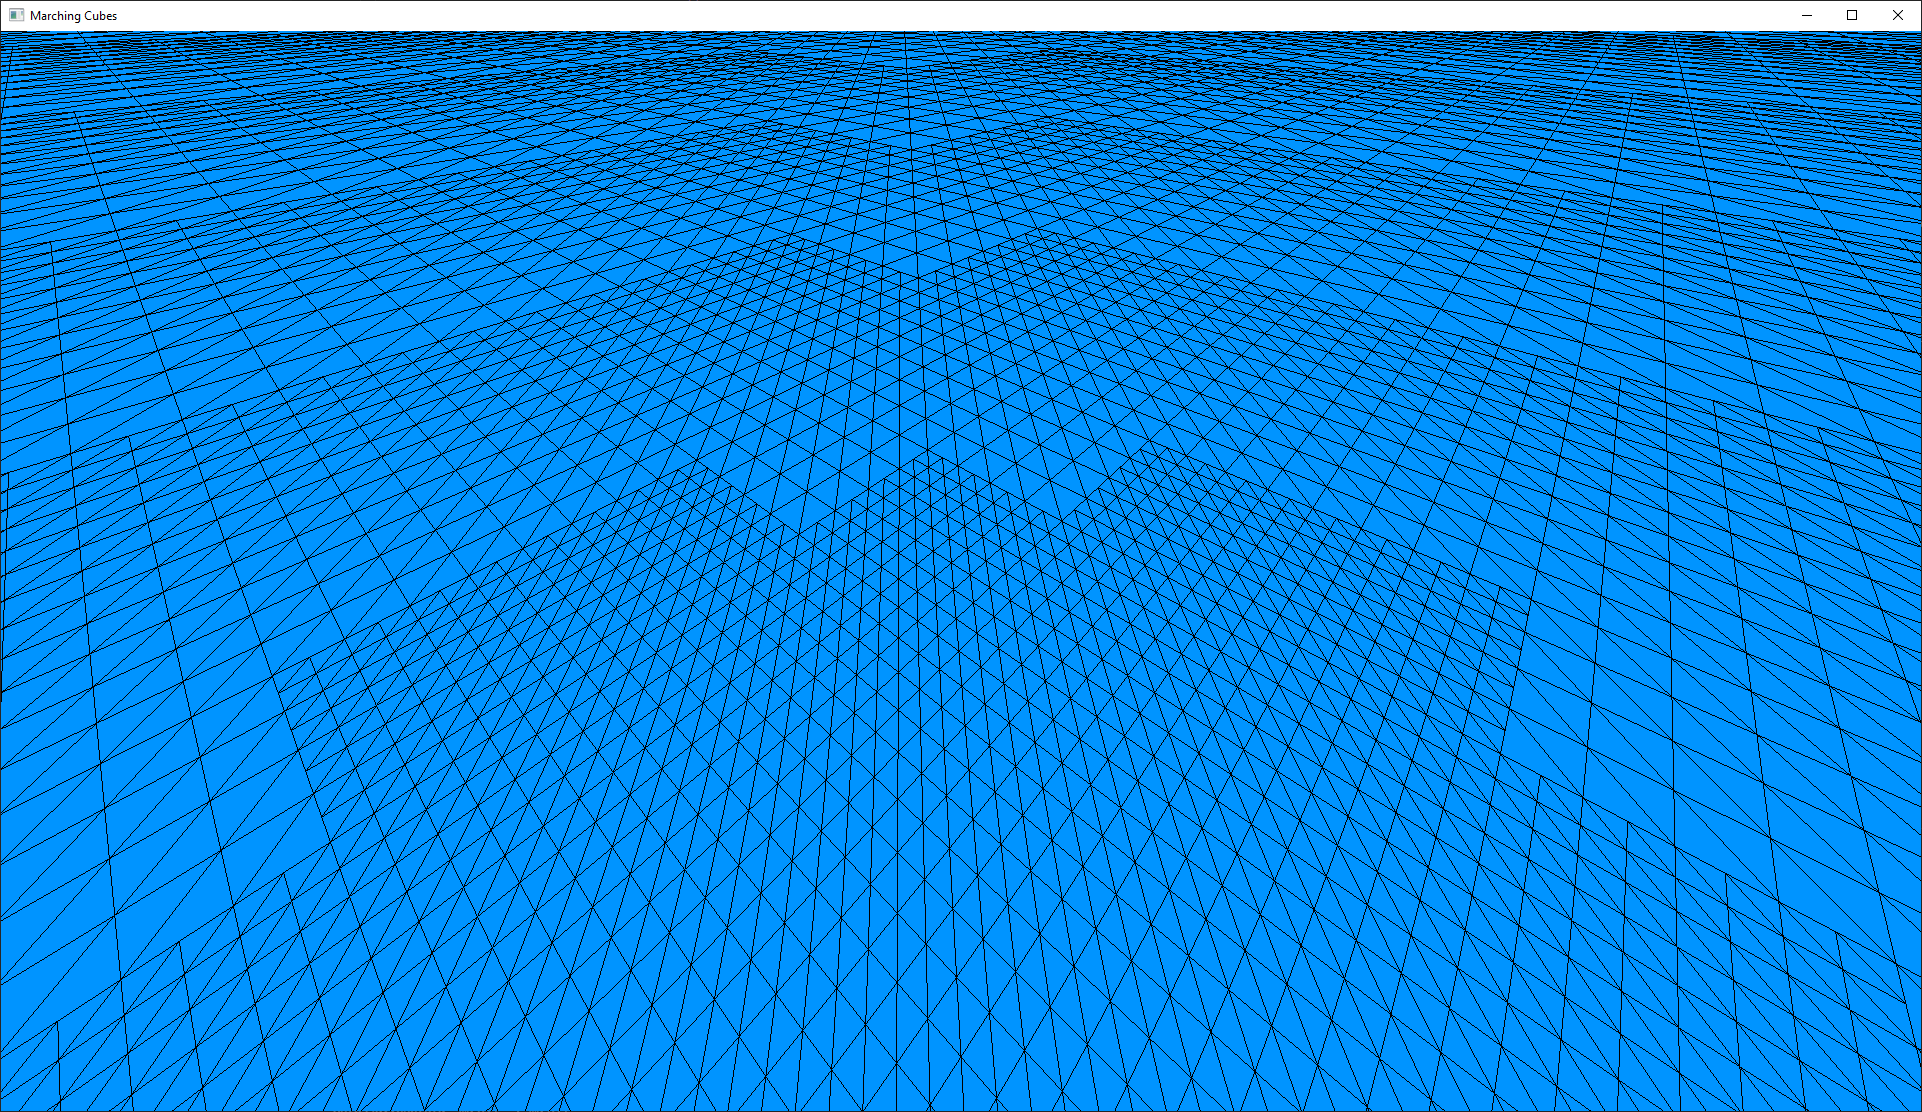
\includegraphics[width=\textwidth]{octree_plane.png}
  \caption{A plane SDF being generated using this octree LOD system. Here, the chunk size is $4^3$. The level of detail is configured to decrease as the distance from the camera increases.}
\end{figure}

When the octree changes, the level of detail at various points changes. The geometry currently generated at those points will be the wrong level of detail, and is considered invalid. The Marching Cubes chunks are deleted, and the region is completely regenerated at the correct level of detail.

\subsubsection{Issue with the Marching Cubes algorithm and LOD systems}
\label{section:cracks}
Using the Marching Cubes algorithm with multiple different grid cell sizes causes undesirable cracks in the surface of the generated geometry on the boundary between chunks of different levels of detail. A demonstration of what causes this is shown in figure \ref{fig:cracks_demo}, and an example within my code is shown in figure \ref{fig:cracks2}.

\begin{SCfigure}[][h]
  \caption{An illustration of the cracks between different levels of detail in the Marching Cubes algorithm. This figure shows the faces of 2 adjacent grid cells. The exact surface represented by the SDF is shown in purple, and the dotted lines show edges that may be produced by the Marching Cubes algorithm at the level of detail of these grid cells, and the level below. When these 2 cases occur next to each other, the space in between the 2 dotted lines forms a crack in the geometry.}
  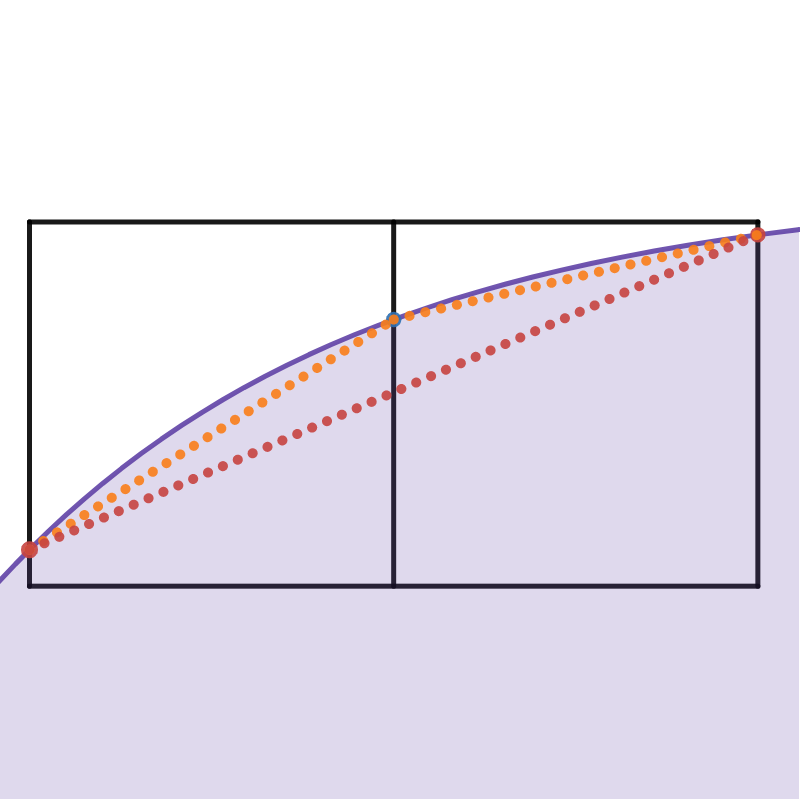
\includegraphics[width=0.5\textwidth]{cracks_demo.png}
  \label{fig:cracks_demo}
\end{SCfigure}

\begin{figure}[H]
  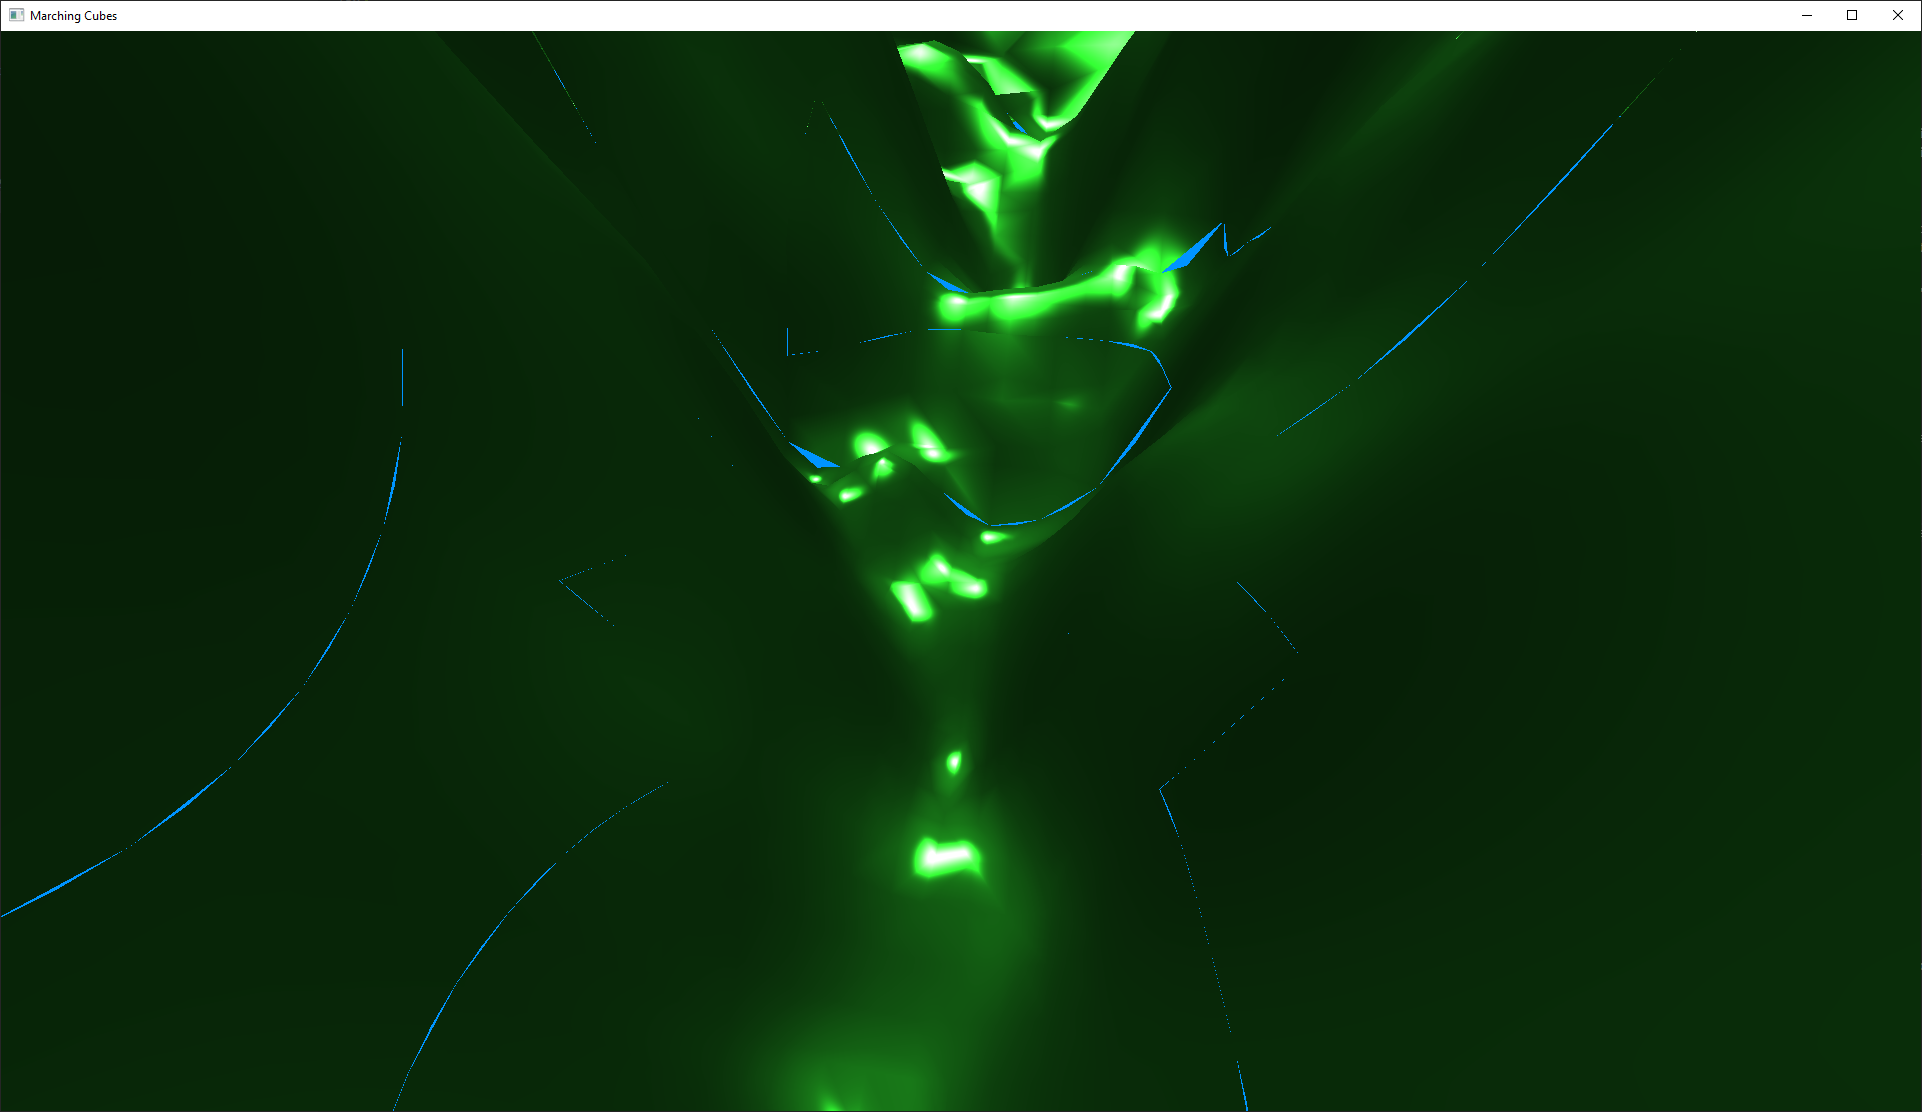
\includegraphics[width=\textwidth]{cracks2.png}
  \caption{An example with low chunk size, where the cracks in between levels of detail are clearly visible.}
  \label{fig:cracks2}
\end{figure}



\subsection{Transvoxel Algorithm}
To solve the problem mentioned in section \ref{section:cracks}, we will switch the algorithm used to generate geometry. The Transvoxel algorithm \cite{lengyel_2010} is an algorithm based on the Marching Cubes algorithm that solves this problem by adding additional vertices into the less detailed mesh, on the faces of Marching Cubes cells adjacent to cells of a higher level of detail. This is done by splitting a cell at the lower resolution (a half-resolution cell) into a regular cell and some amount of transition cells, so that the transition cells border the regular cells at the higher resolution (full-resolution cells). These transition cells need not be cube shaped, and serve as a method of stitching the gap in between half-resolution and full-resolution cells. Figure \ref{fig:transition_cells}, reproduced from the Transvoxel algorithm paper, shows the position of transition cells in 2 different possible configurations.
\begin{figure}[H]
  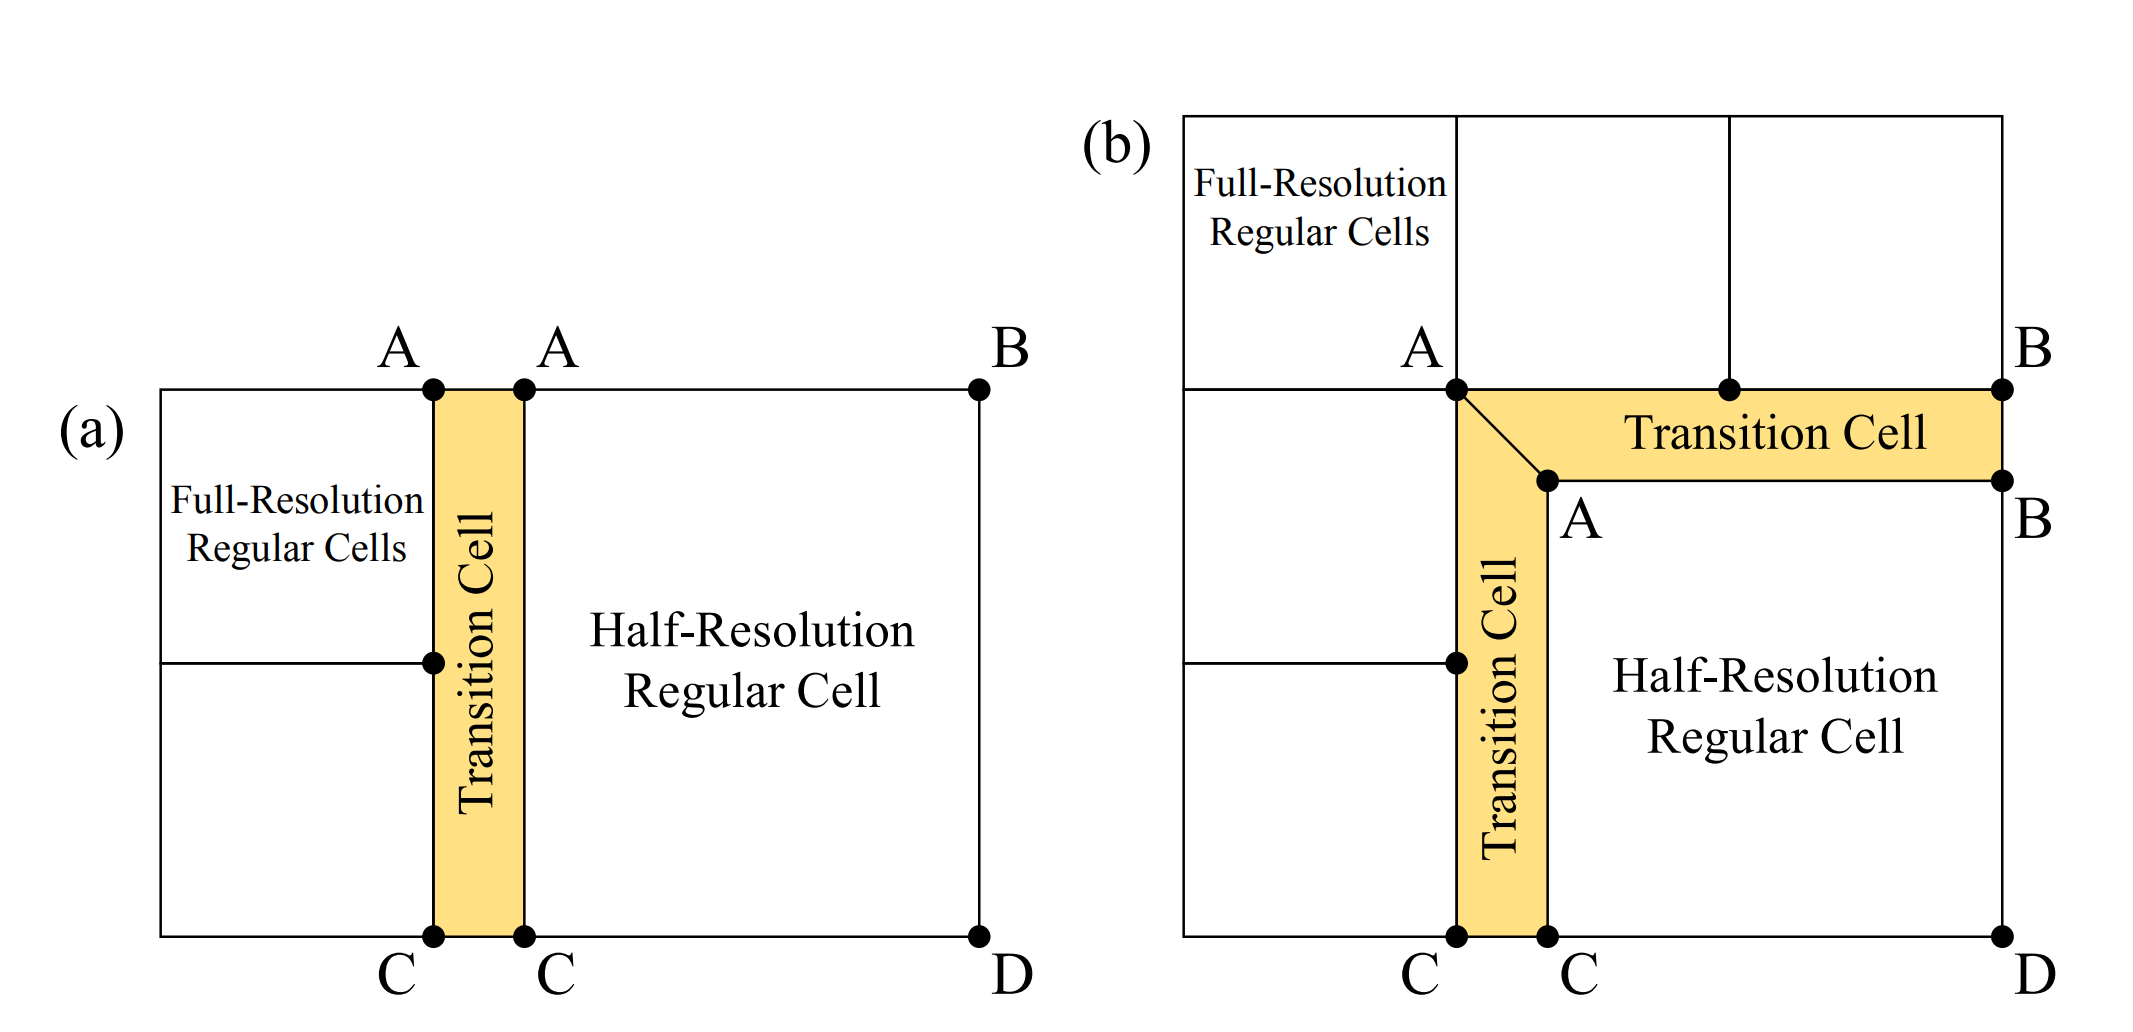
\includegraphics[width=\textwidth]{transition_cells}
  \caption{A 2D illustration of possible configurations of transition cells on the boundary between levels of detail. The half-resolution regular cell has been resized, and the transition cells fit in the space made in between the cells}
  \label{fig:transition_cells}
\end{figure}

The Transvoxel algorithm works similarly to the Marching Cubes algorithm, since it can be implemented to work independently on grid cells. Hence it is also an algorithm that greatly benefits from the parallel processing power of the GPU. The algorithm relies on large lookup tables in a similar way to the Marching Cubes algorithm. For these, we will modify a set of lookup tables provided by the original author of the Transvoxel algorithm \footnote{https://transvoxel.org/Transvoxel.cpp}
\subsubsection{Adaption of the algorithm to GPU}

To parallelise the Transvoxel algorithm, we employ a similar three phase approach to the one described in section \ref{section:mc_gpu}. However, since the algorithm now needs to account for transition cells, and therefore additional SDF sample values, the stages become considerably more complicated. Once again, the algorithm operates on large chunks made up of grid cells, and the resolution of a chunk determines the size of each grid cell. To determine where transition cells need to be generated, a chunk now makes use of a new variable, \texttt{edgeIndex}. This is a 6-bit integer, such that each bit stores whether a face should have transition cells generated on it. This is a parameter passed to the shaders before they are run. The calculation of \texttt{edgeIndex} is described in section \ref{section:edgeIndex}

\begin{enumerate}
\item \underline{Distance function computation}: For each grid cell vertex, sample the SDF. In addition, if this vertex lies on the face of the chunk, also sample the SDF at additional points on the face, for use in transition cells. Store all of these values in a buffer for the next phases. This shader is invoked once for each grid cell vertex, and the invocations corresponding to the vertices on the faces where transition cells are generated are responsible for calculating the additional sample points

\begin{lstlisting}[language=C++,label={tv_generate},caption={Part of the GLSL code responsible for sampling the SDF in the parallel Transvoxel algorithm. This code snippet samples the SDF at the actual grid point, as well as at points surrounding it on the -X and +X facing faces. Lines 7-17 are repeated for the remaining faces of the chunk. Figure \ref{fig:tv_gen_grid} demonstrates which sample points would be calculated in various invocations of this algorithm. The \texttt{generate} function takes 2 parameters: the first is the actual position of the grid cell vertex, and the second is an offset parameter, for generating sample values halfway beetween grid vertices. For example, a value of \texttt{uvec3(0,1,0)} corresponds to a point that is offset from the position in the first argument by half a grid cell in the Y direction.}]
uvec3 gid = gl_GlobalInvocationID;
if (gid.x > chunkSize.x || gid.y > chunkSize.y || gid.z > chunkSize.z) {
  return;
}
generate(gid,uvec3(0));

if ((gid.x == 0 && (edgeIndex & 1) != 0) || (gid.x == chunkSize.x && (edgeIndex & 2) != 0)) {
  if (gid.y < chunkSize.y) {
    generate(gid,uvec3(0,1,0));
  }
  if (gid.z < chunkSize.z) {
    generate(gid,uvec3(0,0,1));
  }
  if (gid.y < chunkSize.y && gid.z < chunkSize.z) {
    generate(gid,uvec3(0,1,1));
  }
}
\end{lstlisting}

\begin{SCfigure}[][h]
  \caption{Illustration of the points that will be sampled on the face of a 2x2x2 chunk when transition cells will be generated. The 4 blue points in the bottom left show the points that will be sampled by an invocation on the vertex at $\left(0,0\right)$, the 2 green points in the bottom right show the points that will be sampled by an invocation on the vertex at $\left(2,0\right)$, and the singular purple point shows the point that will be sampled by an invocation on the vertex at $\left(2,2\right)$. Since this vertex is on the corner of the chunk, no additional points need to be sampled.}
  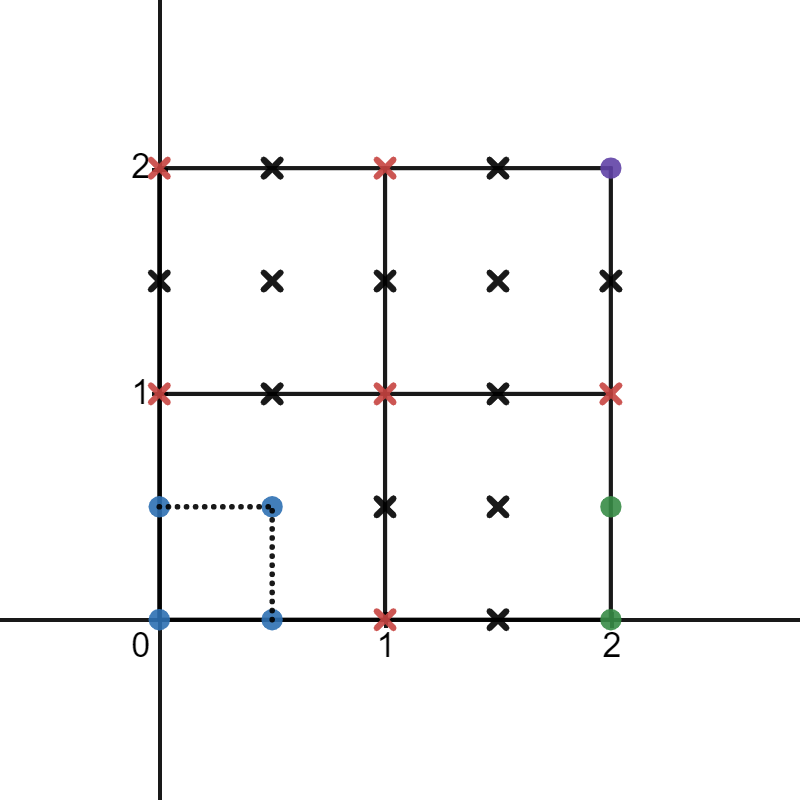
\includegraphics[width=0.5\textwidth]{tv_gen_grid}
  \label{fig:tv_gen_grid}
\end{SCfigure}

\item \underline{Counting phase}: For each grid cell in the chunk, calculate the number of mesh triangles inside the regular cell within it, and if this number is non-zero, add it to the list of cells to generate geometry for in the next phase. This part of the algorithm is the same as the Marching Cubes algorithm. To handle the additional transition cells, the following is done, for each possible orientation of transition cell:
  \begin{itemize}
    \item Check whether a transition cell should be generated, based on \texttt{edgeIndex}, and whether this grid cell lies on the face of the chunk. If not, then skip the rest of the generation.
    \item Determine the values of the SDF on the higher resolution face of the transition cell. This corresponds to the additional values generated on the face in the previous phase. These values determine the geometry that exists within the transition cell. In particular, this does not rely on the values of the SDF on the opposite face of the transition cell. Use this information to calculate the variable \texttt{transitionCellIndex}.
    \item Use the lookup tables with \texttt{transitionCellIndex} to determine how much geometry exists within this transition cell, and increase the atomic counter accordingly.
    \item Append this transition cell to the buffer of cells to be polygonised in the subsequent phase. The transition cell will be polygonised separately from the regular cell that exists within the same grid cell. Additional flags are added to the data in this buffer to indicate that this cell is a transition cell, and its orientation.
  \end{itemize}
\begin{lstlisting}[language=C++,label={tv_count},caption={Part of the code responsible for counting the triangles in transition cells, and appending them to the geometry generation buffer. The first 9 bits of \texttt{paddedTransitionCellIndex} store the type of geometry inside the transition cell, the 10th bit records that the cell is a transition cell, and bits 11-16 are a mask identifying the orientation of the transition cell.}]
//cell is a transition cell:
int paddedTransitionCellIndex = transitionCellIndex;
paddedTransitionCellIndex |= (1<<9);

//store cell orientation:
paddedTransitionCellIndex |= (mask<<10);

//do not march if all inside or all outside
if (transitionCellIndex != 0 && transitionCellIndex != 511) {
  //number of points in the mesh
  //and with 0x7f for lookup table
  atomicCounterAddARB(pointCount,transitionTotalTable[0x7F & transitionCellClass[transitionCellIndex]]);

  uint bufferIndex = atomicCounterIncrement(marchableCount);
  uvec4 mc = uvec4(gid.x,gid.y,gid.z,paddedTransitionCellIndex);
  marchableList[bufferIndex] = mc;
}
\end{lstlisting}

\item \underline{Polygonisation phase}: This shader is run once for each regular cell or transition cell that will contain geometry, as decided by the previous phase. For regular cells, this process is essentially the same as for the regular Marching Cubes algorithm. However, care must be taken to ensure that vertices are placed in the right position. In the case where a regular cell has been made smaller, the SDF has been sampled at the grid cell vertices, rather than the vertices of the regular cell. This introduces inaccuracies in the resulting geometry. The Transvoxel algorithm paper describes a transformation that solves this issue, which is applied to the generated vertices whenever the cell vertices have changed position. Figure \ref{tv_poly_transform} shows the implementation of this transformation.

\begin{lstlisting}[language=C++,label={tv_poly_transform},caption={Transformation to be applied to a generated vertex, when the cell vertices it is being generated between have moved.}]
if (hasShifted[v1Index] || hasShifted[v2Index]) { //if this vertex has moved
  //apply the transformation as in Figure 4.12 in the Transvoxel paper

  //where the vertex would have been
  vec3 vp2 = VertexInterp(gridPos[v1Index],gridPos[v2Index],gridCells[v1Index], gridCells[v2Index]);
  //normal at this position - in world space
  vec3 n = modified_normal(vp2 * chunkStride + chunkPosition);
  vec3 dv = vertPos - vp2;
  vertPos -= (dot(n,dv)) * n;
}
\end{lstlisting}

Transition cells are handled completely separately from the regular cells, even if they share the same grid cell. There are multiple possible shapes a transition cell may need to take, depending on the resolution of surrounding cells, so that they fully close the gaps in between levels of detail. These vertex positions are calculated per transition cell, and the geometry to generate is sourced from lookup tables. Figure \ref{fig:transition_cells} showed some examples of different shapes the transition cell may take, although this does not cover all of the possible shapes. In particular, there is a case where multiple vertices of the transition cell may be moved to the same place. An example of this occuring is shown in figure \ref{fig:tv_transition_plane}. This could lead to zero-width triangles being generated, which is not desirable, and could have the potential to interfere with any other algorithms the generated geometry is used with. However, the number of zero-width triangles is likely to be small, so we simply ignore this issue.

\begin{figure}[H]
  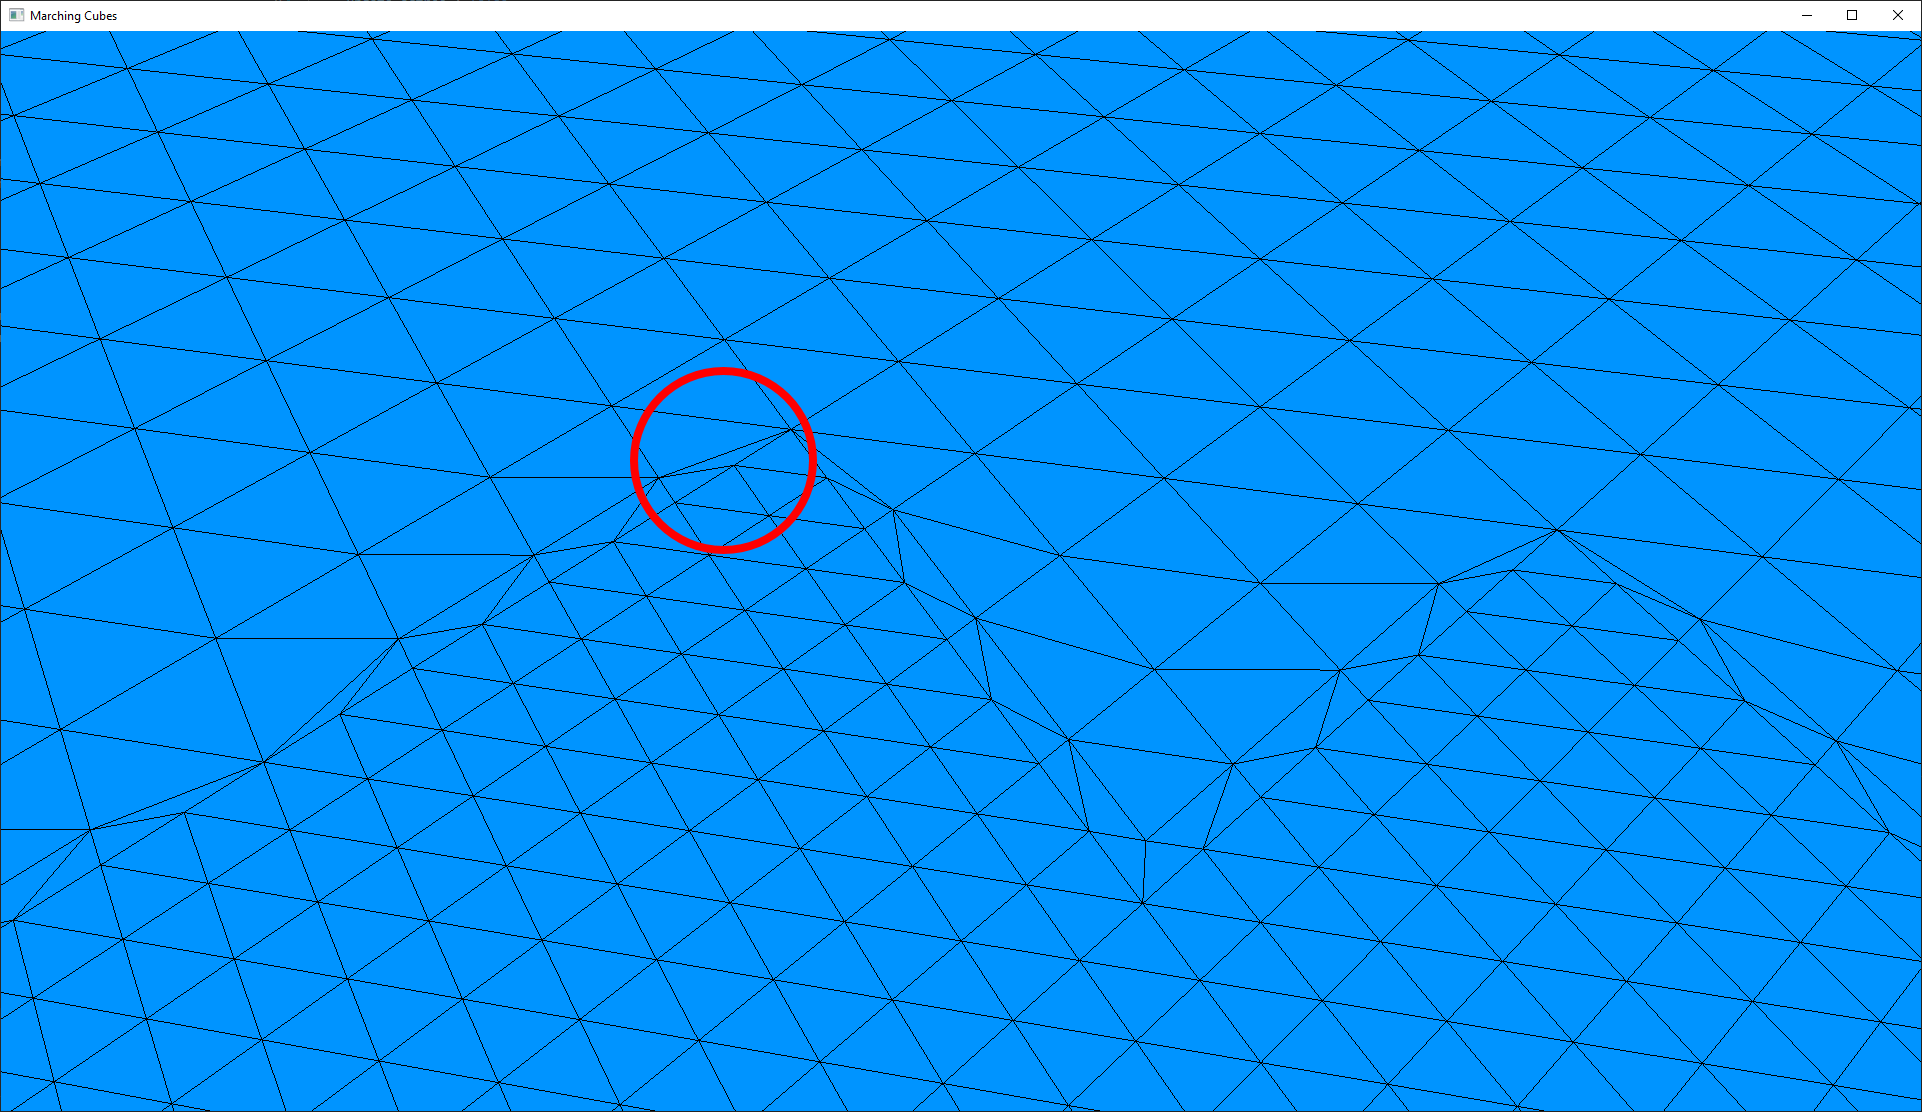
\includegraphics[width=\textwidth]{tv_transition_plane}
  \caption{Example of a plane being generated with Transvoxel transition cells between levels of detail. The circled transition cell has vertices placed on top of each other, leading to zero-width triangles.}
  \label{fig:tv_transition_plane}
\end{figure}

\end{enumerate}

The original Transvoxel implementation contained optimizations for vertex sharing that relied on sequential generation of the geometry. This has been removed from my implementation, for the same reason as described at the end of section \ref{section:mc_gpu}.
\subsubsection{Calculation of edgeIndex}
\label{section:edgeIndex}
For each generated chunk, the variable \texttt{edgeIndex} needs to be calculated. This is done using the octree data structure described in section \ref{section:octree}. For each octree node containing a chunk, the algorithm searches the octree using a recursive algorithm to find neighbor nodes in each direction that exist at the same level of detail. If a neighbor is a leaf, it contains a chunk, and this means the neighboring geometry is at the same level of detail. If no neighbor exists at the same level of detail in some direction, then the neighboring geometry is at a lower level of detail. \texttt{edgeIndex} is not modified in this case, since \texttt{edgeIndex} will be modified for the lower level of detail chunk. If the neighbor is not a leaf, then the neighboring geometry is at a higher level of detail, and edgeIndex is modified to record that transition cells should be generated in that direction. Listing \ref{octree_neighbor} shows the code responsible for finding the neighbors of an octree cell.

\begin{lstlisting}[language=C++,label={octree_neighbor},caption={Code for finding the neighbor of a cell at the same level of detail in an octree. The children of an octree node are stored as a 3D array of pointers to octree objects: \texttt{Octree* myChildren[2][2][2];}. \texttt{relativePosition} is a 3-component vector, where exactly one component is non-zero, corresponding to the direction in which to look for the neighbor. For example, a value of $\left(1,0,0\right)$ searches in the positive X direction, and a value of $\left(0,0,-1\right)$ searches in the negative Z direction.}]
//return the neighbor at the same LOD if one exists, or NULL if none exists
//whether this is a leaf or not determines the edge index
Octree* Octree::getNeighbor(glm::ivec3 relativePosition) {
  if (!myParent) {
      return NULL;
  }
  glm::ivec3 childPosition = relativePosition + glm::ivec3(myPositionInParent);
  if (glm::all(glm::greaterThanEqual(childPosition, glm::ivec3(0))) && glm::all(glm::lessThanEqual(childPosition,glm::ivec3(1)))) {
    //return the parent child at this relative position
    return myParent->childFromVec3(childPosition);
  } else {
    //return the child of the parent neighbor
    Octree* neighbor = myParent->getNeighbor(relativePosition);
    if (!neighbor || neighbor->isLeaf) return NULL;
    //glm does not have integer mod, so we have to do this manually...
    glm::ivec3 cm2 = glm::abs(glm::ivec3(childPosition.x % 2, childPosition.y % 2, childPosition.z % 2));
    return neighbor->childFromVec3(cm2);
  }
}
\end{lstlisting}

\begin{SCfigure}[][h]
  \caption{The blue cell has 3 neighbors at the same level of detail. The green neighbor is within the same parent octree cell, and no recursive calls are needed. The red neighbor is not within the same parent cell, so the neighbor of the parent is found, and the corresponding child of this neighbor is returned. The orange neighbor is not a leaf, so \texttt{edgeIndex} is updated to reflect this. There is no neighbor at the same level of detail above the blue cell.}
  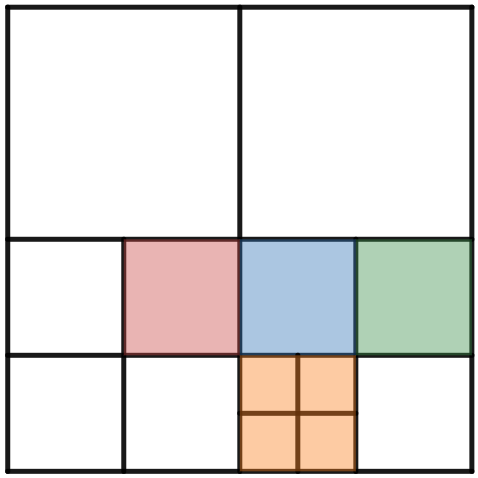
\includegraphics[width=0.5\textwidth]{octree_neighbors.png}
  \label{fig:octree_neighbors}
\end{SCfigure}

This approach is sufficient in most cases for eliminating cracks in the geometry. However, there are still octree configurations which could occur, where different levels of detail appear next to each other, even once transition cells have been generated. Figure \ref{fig:octree_neighbor_error} shows an example of when this can occur.

\begin{SCfigure}[][h]
  \caption{An example octree configuration where different levels of detail may occur next to each other, even with transition cells. Areas where transition cells will be generated are shaded in blue. The area where transition cells may be generated, but different levels of detail will still be adjacent to each other, is shaded in red. Directly below this region are regions that are 2 levels of detail higher than the cell for which transition cells have been generated.}
  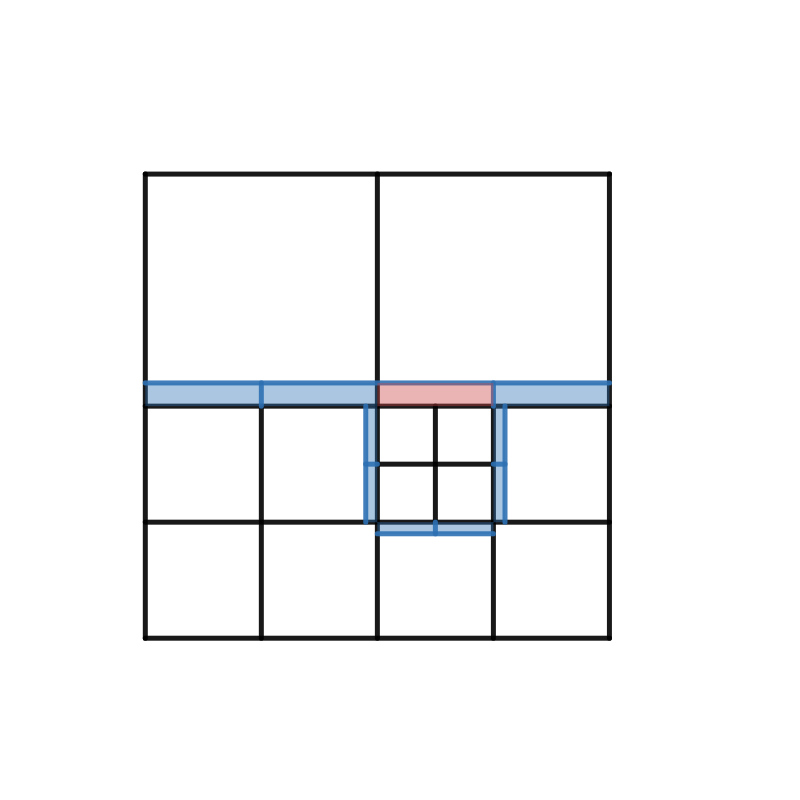
\includegraphics[width=0.5\textwidth]{octree_neighbor_error.png}
  \label{fig:octree_neighbor_error}
\end{SCfigure}

To rectify this issue, a refinement strategy is used to ensure that cases like this do not occur within the octree. When the octree needs to be modified, the following 4 steps are performed in order:
\begin{enumerate}
  \item Traverse the octree data structure, visiting every node, including leaves. If a node satisfies \texttt{shouldChop}, then flag it, but do not delete its children yet. If a node satisfies \texttt{shouldSplit}, then split it, creating the 8 new leaf nodes. The newly created leaf nodes will also be traversed in this step, since this allows for more than one layer of the octree to be generated at once.
  \item If the first step changed the structure of the octree, or flagged any nodes, then traverse the octree, checking whether any nodes have neighbors which are more than one level of detail higher. This is done using the \texttt{getNeighbor} function described in listing \ref{octree_neighbor}. If this occurs, then split the node into its 8 children. If the node is not a leaf, but was flagged by the previous phase, the unflag it. This flagging prevents octree nodes and the geometry chunks that have been created as a result of this refinement being deleted in the first step, then immediately recreated. Performing this refinement step may create inconsistencies elsewhere. Hence, it is performed repeatedly, until no changes are made.
  \item Once the previous step is complete, traverse the octree, deleting the children of any nodes which are still flagged. Since this step reaches all of the leaves of the updated octree structure, and does not create additional leaves, it is also where any regeneration of geometry chunks occurs, if this is necessary (for example, if the geometry inside the chunk has been modified).
  \item Traverse the octree a final time, generating geometry chunks for all new leaves, and all leaves that needed regeneration. Also regenerate geometry for all leaves where \texttt{edgeIndex} has changed, so that cracks do not appear after changing the level of detail of a neighboring chunk.
\end{enumerate}
Listing \ref{octree_refine} shows the code responsible for this:
\begin{lstlisting}[language=C++,label={octree_refine},caption={Code showing the order of steps in the octree refinement process}]
void Octree::refresh(glm::vec3 inPos) {
  //Initially, pass through the entire octree and flag chunks that should be deleted, according to the chop condition
  //Or split, according to split condition
  //return true if something has split
  bool needsRefinement = flagSplitPhase(inPos);

  //Refine, undoing flags rather than splitting
  //need many passes, because a refinement may cause inconsistencies elsewhere
  if (needsRefinement) {
    bool done = false;
    int steps = 0;
    while (!done) {
      steps++;
      done = refine();
    }
  }
  //Now delete flagged chunks. Since this reaches all leaves, also do editing regeneration here
  deleteRegenPhase();

  generateAllChunks();
}
\end{lstlisting}


\subsubsection{Efficiency compared to Marching Cubes}
% todo - make this efficient
- TODO: regardless, this is still pretty fast on the GPU\\

\subsection{Terrain Modification}
\subsubsection{Method of Terrain Modification}
Since the parallel Transvoxel algorithm runs so efficiently, it is possible to regenerate significant portions of geometry in between frames, and so real-time terrain editing is achievable.\\
There are multiple different approaches to modifying the generated geometry. Modifying the generated geometry, for example by dragging or inserting vertices, edges and faces, is possible, however is a subsequent step applied after the Transvoxel algorithm, and the modifications would be ambiguous when the level of detail changes. Alternatively, the value of the SDF at sample points could be modified. This would give an effect of pushing the geometry in or pulling it out, at a point. However, this sort of modification would also be ambiguous when the level of detail changes. The approach we will use will be to add primitive shapes to the SDF itself, using the set-theoretical operations, and their representations as discussed in section \ref{section:sdf}. This means that the shape represented by the SDF changes, so the generated geometry also changes, regardless of the level of detail.
\subsubsection{Implementation of Primitives}
 - how are they actually implemented\\
 - bounding boxes of primitives - dont need to evaluate parts not affected\\
 - Example of simple shape, and more complex ones eg bezier\\
 - bezier approximation vs exact\\
\subsubsection{Regeneration of Chunks}
 - regenerating chunks\\
 - when to regenerate chunks, and which ones\\
\subsubsection{Limits of terrain modification}
 - how many primitives is reasonable before slowdown due to SDF evaluation?\\
 %TODO - GUI
 
 \subsection{Physics}
 To implement physics collision with the generated geometry, we use a well-known library called Bullet Physics. This library contains many built-in optimisations for efficient collision detection between meshes. %TODO - citation for this
 - mapping geometry from GPU to CPU?
 - zero-width triangles havent turned out to be a problem so far\\
 - generating physics meshes is slow - need to find a solution to this\\
 - In fact, physics is currently the *slowest* part of this...\\
 \subsubsection{Multithreading}
 To enable physics meshes to be generated whilst maintaining an interactive framerate, they are generated on a separate thread. However, this introduces race conditions between the main thread, which iterates over physics objects in the world, and the thread on which the meshes are generated. Furthermore, if a chunk is deleted by the main thread (such as when the level of detail changes, or when the SDF has been modified), whilst the physics mesh is being generated by another thread, then the mesh generation will fail, and likely cause the program to crash by attempting to access deallocated memory. To solve this problem, the state of a chunk mesh is carefully maintained throughout its lifetime, with defined transitions between states occuring where race conditions may occur. % TODO - improve this?
 \begin{figure}[H]
  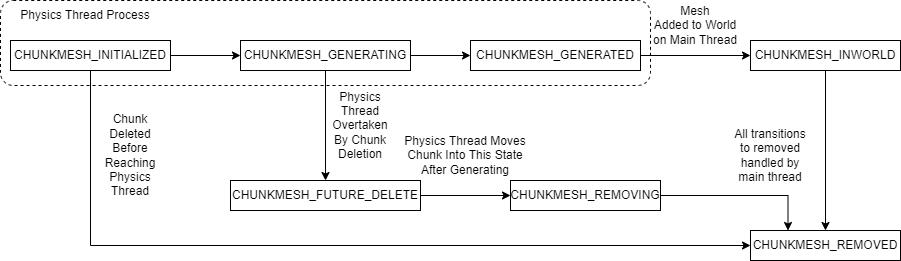
\includegraphics[width=\textwidth]{physics_states.png}
  \caption{States of a physics mesh}
  \label{fig:physics_states}
\end{figure}
 \subsubsection{SDF-based physics}
 - perhaps look at this - might be a struggle because of non-exact SDFs, and how would we do it for anything that isn't a sphere anyway?
 
 \section{Implementation}
  - C++ with fairly low-level opengl libraries\\
  - key code probably in design section already\\
  - section for the ``boring bits'' of the implementation, rather than key ideas\\
  - perhaps section to explain other things that needed bugfixes?\\
  - something tying it all together?
  
\section{Conclusion}
 - demonstration of final product\\
 - conclusion\\
 - somehting about future work?

%\paragraph{paragraph}
%\subparagraph{subparagraph}

\bibliography{mc}
\end{document}